%# -*- coding: utf-8-unix -*-
%%==================================================
%% chapter02.tex for SJTU Master Thesis
%% Encoding: UTF-8
%%==================================================

\chapter{电路拓扑符号化自动降阶模型生成方法}
\label{chap:simp}

上一章介绍了电路模型对电路设计的重要性,可见电路低阶模型本身的提出也应有一定方法可以指导其生成。
只有在拥有可靠的模拟集成电路低阶模型的情况下,电路设计工程师才有可能对电路做出进一步的理论分析,从而指导进一步的设计。
本章给出了本文最关键的算法:采用拓扑简化方法得到的低阶模型自动生成算法,并给出了其相关的测试结果,佐证了算法的有效性。

\section{双图决策树符号约简}
\label{sec:simp:GPDD}

\subsection{电路元件极值与元件拓扑的关系}
\label{subsec:simp:GPDD:TopoLimit}

本课题采用拓扑简化的方法实现电路模型的自动生成。
所以电路元件的拓扑结构对于分析本身有非常重要的作用。
我们发现电路的元件的极限取值可以代表新的简化的电路拓扑结构。
这正可以成为我们对电路简化的基石。
当我们考虑需要将一个电路中的元件删去时,即可认为是电路这个元件选取了极限的取值导致。
当然一个电路元件删去过程中,往往存在两个电路元件删去方式:短路和断路。

\begin{figure}[!htp]
	\centering
	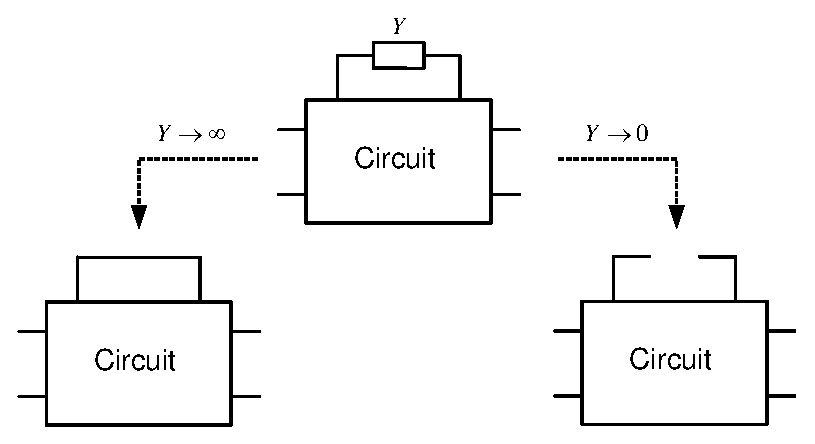
\includegraphics[width=0.7\textwidth]{chap2/LimitTopo.eps}
	\bicaption[fig:limittopo]{导纳在极限取值情况下的拓扑结构改变}{导纳在极限取值情况下的拓扑结构改变}{Fig}{Topological adjustment of impedance whose value changes to limit value}
\end{figure}

如图\ref{fig:limittopo}所示,假设在一个电路中有一处导纳值为$Y$的阻抗。
现在我们用两个极限的值$\infty$和$0$去替代这个导纳值$Y$。
可以看到当,导纳值$Y$趋向于无穷大时,由于此时其相应的阻抗$Z$为零,所以此时这个阻抗变为短路的电路结构;
然而当导纳值$Y$趋向于零时,由于此时其阻抗值$Z$为无穷大,这种情况下电路结构变为阻抗两端的两个节点变为了断路的状态。
可以看到,这样我们就可以用电路元件的极限取值来替代线性阻抗元件(R/L/C)的拓扑变化。

然而,在小信号电路中,我们知道不仅存在线性阻抗元件(R/L/C),另外还有四种受控信号源,分别为:电压控制电压源(VCVS),电流控制电流源(CCCS),电压控制电流源(VCCS),电流控制电压源(CCVS)。
我们发现在以上两种极限取值仍然适用于这四种受控源,特别是在取无穷大情况下,它们都会成为一种称为Nullor的电路元件,如图\ref{fig:nullor}。

\begin{figure}[!htp]
	\centering
	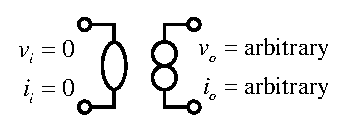
\includegraphics[width=0.35\textwidth]{chap2/SymbolNullor.eps}
	\bicaption[fig:nullor]{Nullor元件符号}{Nullor元件符号}{Fig}{Nullor symbol}
\end{figure}

可以看到,Nullor元件假设其输入端的输入电流和电压均为0,有着任意大小的输出能力。
Nullor这种元件与传统的模拟电路学习中接入负反馈中的理想运算放大器的虚短虚断的性质是一致。
但由于Nullor本身往往可以与电路中别的元件合并,并且不会出现在电路最后的模型中,这一点会在本章中节\ref{subsubsec:simp:res:cir:fd}中看到。

\begin{table}[!htbp]
	\bicaption[tab:symbollimit]{电路元件极限取值的拓扑结构}{电路元件极限取值的拓扑结构}{Table}{Circuit element topology whose value is infinity or zero}
	\centering
	\begin{tabular}{c|c|c}
		\hline
		\multirow{2}{*}{Symbol} & \multicolumn{2}{c}{Value}\\
		\cline{2-3} 
		& $\infty$ & $0$\\
		\hline
		\parbox[c]{0.11\textwidth}{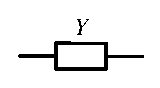
\includegraphics[width=0.11\textwidth]{chap2/Impedance.eps}} & 
		\parbox[c]{0.11\textwidth}{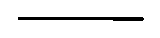
\includegraphics[width=0.11\textwidth]{chap2/Impedance-Short.eps}} & 
		\parbox[c]{0.11\textwidth}{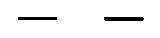
\includegraphics[width=0.11\textwidth]{chap2/Impedance-Open.eps}} \\
		\hline
		\parbox[c]{0.2\textwidth}{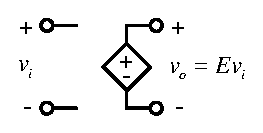
\includegraphics[width=0.2\textwidth]{chap2/VCVS.eps}} & 
		\parbox[c]{0.11\textwidth}{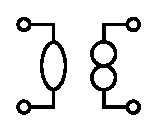
\includegraphics[width=0.11\textwidth]{chap2/Nullor.eps}} & 
		\parbox[c]{0.11\textwidth}{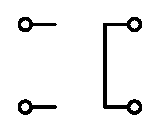
\includegraphics[width=0.11\textwidth]{chap2/VCVS-Open.eps}} \\
		\hline
		\parbox[c]{0.2\textwidth}{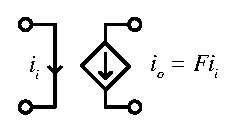
\includegraphics[width=0.2\textwidth]{chap2/CCCS.eps}} & 
		\parbox[c]{0.11\textwidth}{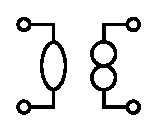
\includegraphics[width=0.11\textwidth]{chap2/Nullor.eps}} & 
		\parbox[c]{0.11\textwidth}{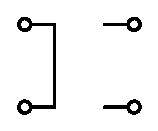
\includegraphics[width=0.11\textwidth]{chap2/CCCS-Open.eps}} \\
		\hline
		\parbox[c]{0.2\textwidth}{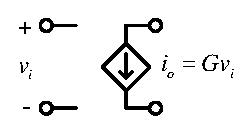
\includegraphics[width=0.2\textwidth]{chap2/VCCS.eps}} & 
		\parbox[c]{0.11\textwidth}{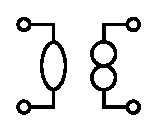
\includegraphics[width=0.11\textwidth]{chap2/Nullor.eps}} & 
		\parbox[c]{0.11\textwidth}{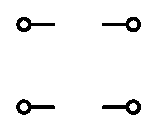
\includegraphics[width=0.11\textwidth]{chap2/VCCS-Open.eps}} \\
		\hline
		\parbox[c]{0.2\textwidth}{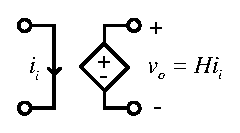
\includegraphics[width=0.2\textwidth]{chap2/CCVS.eps}} & 
		\parbox[c]{0.11\textwidth}{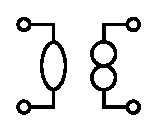
\includegraphics[width=0.11\textwidth]{chap2/Nullor.eps}} & 
		\parbox[c]{0.11\textwidth}{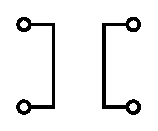
\includegraphics[width=0.11\textwidth]{chap2/CCVS-Open.eps}} \\
		\hline
	\end{tabular}
\end{table}

为了说明受控源取极限值情况下电路拓扑结构的变化,这里仅以VCVS为例进行说明。
所有小信号分析中用到的阻抗和四种受控源的拓扑变化可以参考表\ref{tab:symbollimit}。
我们知道VCVS的输入输出电压关系如下式所示:

\begin{equation}
	v_o = E v_i
\end{equation}

这里,$v_i$和$v_o$分别为VCVS的输入输出电压,$E$则为VCVS的放大倍数。
首先我们考虑$E$取无穷大的情况,为了电路仍然能正常工作,我们知道输出电压$v_o$应为有限值,而其中$E$为无穷大,那么根据基本微积分的知识,我们知道此等式中的输入电压$v_i$为零。
另外由于VCVS的输入端测量电压,所以本来就限定输入的电流$i_i$为零,所以其形成了Nullor的虚短虚断的性质。
另外当$E$的取值为零时,根据VCVS本身的关系,即可得出输出端电压为零,所以输出端两端电压一致,即此端口可用一根导线连接起来,加之本为断路连接的输入端,故VCVS可约减为表\ref{tab:symbollimit}中的结构。

\subsection{双图决策树和电路拓扑的关系}
\label{subsec:simp:GPDD:TopoGPDD}

上一小节已经将电路的极限取值与电路的拓扑结构变化建立起了联系,而此时电路元件的极限求值成为了新的问题。
由于在整个算法过程中,需要多次计算不同拓扑结构下电路性能表现,这要求了高效的计算方法的支持。
然而GPDD结构本身蕴含了对电路拓扑结构,可以轻松方便地在其中对不同的电路拓扑结构求值,这支持了下一节所介绍的简化算法。

\begin{figure}[!htp]
	\centering
	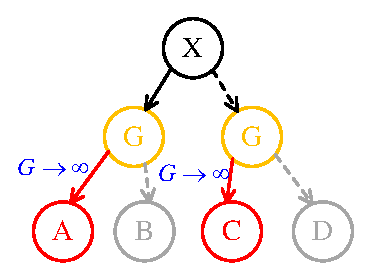
\includegraphics[width=0.35\textwidth]{chap2/GPDDTopo.eps}
	\bicaption[fig:GPDDTopo]{符号极限取值情况下GPDD的计算方法}{符号极限取值情况下GPDD的计算方法}{Fig}{Calculation rule for GPDD under limit value}
\end{figure}

我们知道根据电路基本原理,并且结合GPDD的计算规则,针对类似图\ref{fig:GPDDTopo}这样的GPDD结构,我们可以求得类似下式的电路传输函数表达式(为了说明的方便,这里忽略了GPDD中连接节点的边上的符号):

\begin{equation}
H \left( s \right) = \frac{{{f_A}\left( A \right)G + {f_B}\left( B \right)}}{{{f_C}\left( C \right)G + {f_D}\left( D \right)}}
\end{equation}

考虑目前我们需要对电路中的元件$G$求取极限值,并计算新的符号化传输函数公式。
这里假设元件$G$位于GPDD符号表中的第一层,这里层数不影响极限取值的计算,只是为方便说明特意假设。
我们可以得到在$G$元件取无穷大情况下,电路的新传输函数为:

\begin{equation}
\label{eq:simpGPDD}
\mathop {\lim }\limits_{G \to \infty } H \left( s \right) = \frac{{f_A}\left( A \right)}{{f_C}\left( C \right)}
\end{equation}

首先,十分显然地,可以看到取极限后首先原有的符号$G$从公式消失了,这也暗示了电路拓扑的简化,即$G$从电路中以短路的方式被删去了。
另外,可以发现,在式\ref{eq:simpGPDD}中所有的保留下的符号项均是在GPDD结构中以红色实线相连的红色节点$A$和$C$的值。
由于,我们知道,GPDD结构中实线相连的节点均采用乘法进行计算,故在求取极限的过程中,其相应的系数得到保留。
故当某一符号元件需取无穷大情况下的值时,在GPDD计算过程中,仅需计算GPDD对应符号所有节点左儿子的值即可,所有的右儿子忽略。
同样的,我们知道当对一个电路元件取值零时,GPDD计算中仅需考虑该元件所有节点右儿子的值即可,左儿子的值则忽略,而且算法设计简单,仅需直接用0带入符号值即可。
总结来说,GPDD中某个节点左儿子承担了该节点符号取值无穷大情况(阻抗短路,受控源Nullor)下的电路性能,而右儿子为该节点符号取值零情况(阻抗断路,受控源删去)下的电路性能,当符号本身有一定值时,则为两者的折衷。

当然需要注意的是,在求某一个符号为无穷大时,由于特殊的GPDD规模缩小的算法,类似Reduction、Zero-Suppression等算法\parencite{GShi-GPDD-2013,GShi-GPDD},可能存在有排序在$G$之上的符号直接与排序在$G$之下的符号节点相连的情况。
这种情况需特别注意,因为这种项中不包含$G$符号,故取极限值时,并非系数,也需忽略。
具体的GPDD中符号约减下的计算方法已在\parencite{HanbinHu-Thesis}有阐释,这里不再赘述。

下面通过一个例子展示电路拓扑结构变化对GPDD结构的影响,以直观了解这两者之间的关系。

\begin{exmp}
RLC电路向RC电路简化过程中GPDD结构比较

图\ref{fig:RLC}中展示了一个RLC串联的简易电路,与之前给出的图\ref{fig:RC_cir}相比较,这里多出了电感元件。
可以看到如果这个电感$L$如果取值为零,那么其导纳$Y=\left(s L\right)^{-1}$,即导纳为无穷大情况,即可得到RC电路的电路图。

\begin{figure}[!htp]
	\centering
	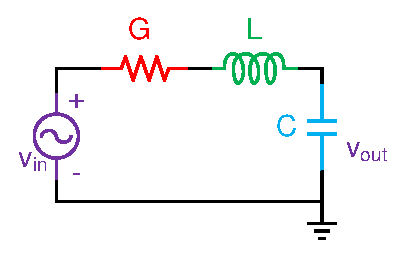
\includegraphics[width=0.4\textwidth]{chap2/RLC.eps}
	\bicaption[fig:RLC]{RLC电路示意图}{RLC电路示意图}{Fig}{RLC circuit example}
\end{figure}

此RLC电路对应的GPDD结构展示在图\ref{fig:RLCvsRC}中的左侧。这张图右侧是展示的RC电路对应的GPDD结构。
可以看到通过两侧曲线包围起来的结构是一致的,而且均与电感符号$L$的左儿子相连,这与之前的论述是相符的。
同时可以看到,由于RC的GPDD结构蕴含在RLC的GPDD结构中,故可以直接在RLC的GPDD结构上对RC电路的GPDD进行求值。
这表示了GPDD拥有在同一个BDD数据结构中求解多种不同电路拓扑的能力,这大大方便了符号简化电路自动生成算法的设计。
这种能在同一个符号化结构中表达不同拓扑结构电路的能力是别的符号化方法不具备的,也是GPDD相比其他的符号化方法一大优势所在。

\begin{figure}[!htp]
	\centering
	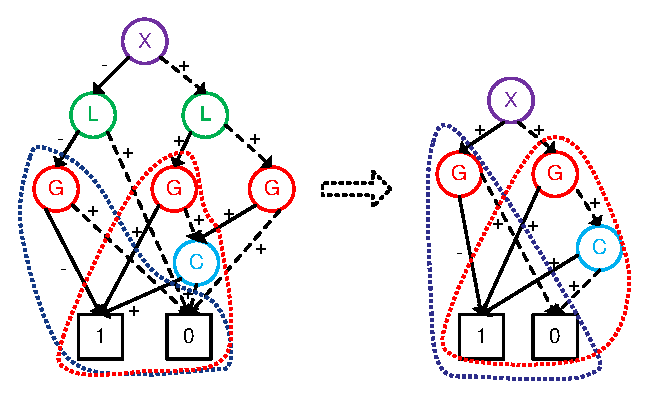
\includegraphics[width=0.7\textwidth]{chap2/RLCvsRC.eps}
	\bicaption[fig:RLCvsRC]{符号极限取值情况下GPDD结构示例}{符号极限取值情况下GPDD结构示例}{Fig}{GPDD structure example under limit value}
\end{figure}

\end{exmp}

GPDD对降阶模型的求解的优势在于在一次符号表达构造的情况下,可以在多次同一个结构中求得对应与不同简化模型的电路传输函数。
符号化构造往往大量计算时间花费在符号化表达式的构造上,而其求值往往是高效的稳定的。
故可以如将构造的时间平摊在之后的多次求值上,仍然得到了许多计算上的便利。
同时,如采用传统的数值化求解器,需要对电路矩阵做行列合并等操作,操作复杂。

\section{符号化降阶模型生成算法与流程}
\label{sec:simp:alg}

在建立电路拓扑与元件取值之间的关系,并使用GPDD这个便利的工具可方便求取电路拓扑变化情况下的电路性能的条件下,本节对符号化降阶模型生成算法进行全面的介绍。
首先,将介绍算法的总体流程,并逐一介绍其中每个流程具体细节,并给出简化过程中一些特殊情况的处理。
本文讨论中,我们主要针对运算放大器的设计进行讨论,故我们接下来的讨论将均针对运算放大器设计。

\subsection{简化算法总体流程}
\label{subsec:simp:alg:top}

降阶模型的建立,我们将其看作一个电路拓扑元件简化的过程,总的流程可参见图\ref{fig:SimpProcedure}的流程示意。

\begin{figure}[!htp]
	\centering
	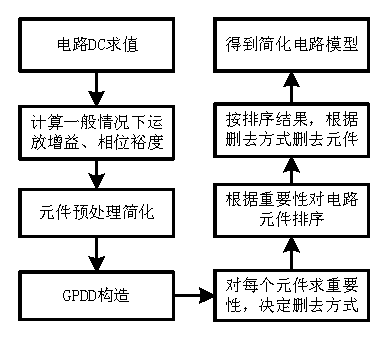
\includegraphics[width=0.5\textwidth]{chap2/SimpProcedure.eps}
	\bicaption[fig:SimpProcedure]{降阶模型自动生成整体流程}{降阶模型自动生成整体流程}{Fig}{Entire procedure for low-order model generation}
\end{figure}

该流程图中有两处以红色斜体标出将在接下来的两个小节\ref{subsec:simp:alg:pre}和\ref{subsec:simp:alg:significance}中详细介绍。
这里先针对其余的部分给出说明。

在拿到一个模拟运放电路后,首先通过数值化仿真器(如:HSPICE)利用DC求解对电路进行求解,以获得电路中所有非线性元件(如:MOSFET)的小信号参数。
接下来,对于完整电路进行AC分析,求得相应的运放增益$A_0$和单位增益频率处相位$PM_0$(即相位裕度处),这两个值将在接下来的元件重要性求值运用到。
对于电路元件进行预处理,做一定粗糙的简化工作,这一步对于生成的最后的简化小信号模型的易于理解性方面有关键的作用,将在\ref{subsec:simp:alg:pre}中具体介绍。
根据初步得到的小信号模型电路,进行GPDD符号化结构的构造,以方便下一步的元件重要性计算。

这里我们定义了电路元件的重要性,某个符号的重要性意味着该电路元件符号对电路性能具有比较大的贡献。
故高重要性的电路元件应予以保留,而低重要性的电路元件应予以删去,故如流程中所示,需要对元件的重要性进行排序。
同时根据前几节的论述,一个符号有两种删去方式,分别为将该元件置为零或无穷大。
我们在计算重要性的过程中即刻确定对应的删去方式,并最终在简化模型生成中以相应的删去方式删去电路元件,从而得到降阶的符号化模型。

这里有一个问题是模型需要多大精度,从而会决定简化的电路模型中保留多少相应的元件。
在目前的研究进程中,我们仅人为指定需要保留多少电路元件,通过人为观察电路频率响应曲线,来决定当前的模型是否合适。

这种简化方法可以看到在符号化构建GPDD后,最关键的时间复杂度主要集中在对元件重要性求值的这一步上。
别的步骤虽然也有一定的时间损耗,但根据我们的实践经验,相比重要性求值步骤来说可以忽略不计。
重要性求值需要对每个电路元件进行计算,故若一个电路中有N个电路元件,构造得到的GPDD结构共有$\left|GPDD\right|$节点。
在\ref{subsec:simp:alg:significance}中可以看到单个元件的重要性求值需$O\left(\left|GPDD\right|\right)$的时间复杂度。
故简化流程的时间复杂度主要由$O\left(N\left|GPDD\right|\right)$决定。

\subsection{元件预处理过程}
\label{subsec:simp:alg:pre}

之所以要对电路进行预先简化,其主要目的在于能够事先将一些信号不通过的节点识别出来,从而事先删去一些节点和元件,方便进一步简化算法。
许多电路从理论上分析,往往会有一定的做法;然而在实际操作中,人们往往会进一步加入自己的理解与分析,从而改变理论分析的结果,虽然过程中隐去了一些电路结构,却使进一步的分析与电路理解更加便利。
这一点在后续的测试结果中也有所体现。
这里以模拟电路中常见的由于输入差分对所造成的虚拟地作为例子,说明这种情况。

\begin{exmp}
虚拟地理论分析与实际操作区别

\begin{figure}[!htp]
	\centering
	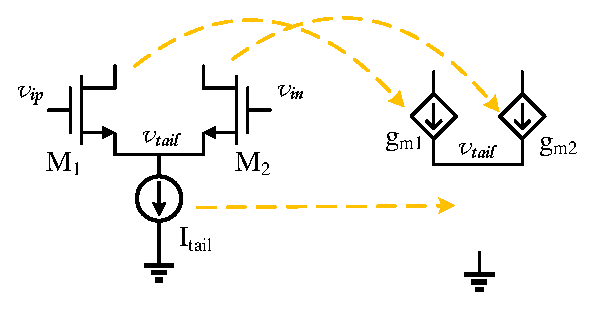
\includegraphics[width=0.6\textwidth]{chap2/VG.eps}
	\bicaption[fig:VG]{虚地的产生原因}{虚地的产生原因}{Fig}{Virtual ground illustration}
\end{figure}

可以看到,图\ref{fig:VG}中展现了经典的模拟电路输入差分对,这样的电路结构一般由一个电流源作为两个输入管的偏置,输入结构两端对称。
在这种结构下,根据传统的电路分析技巧,我们可以画出如图\ref{fig:VG}右侧的小信号结构。
其中理想电流作为断路,所以$v_tail$这一电路节点浮空,同时保留这里的两个MOS管的$g_m$电流源。
我们可以根据$v_tail$这一电路节点的KCL关系,可列写方程有:

\begin{equation}
g_{m1}\left(v_{ip}-v_{tail}\right)+g_{m2}\left(v_{in}-v_{tail}\right)=0
\end{equation}

由于两端的对称性我们知道$v_{ip}=-v_{in}$,并且$g_{m1}=g_{m2}=g_m\neq0$,那么有

\begin{equation}
g_{m} v_{tail} = 0 \Rightarrow v_{tail} = 0
\end{equation}

所以由于尾电流的节点往往被作为虚拟地的存在,在电路分析中往往直接将这一点接到地上,而不是像小信号分析中将电路节点浮空。
这种看似矛盾,实际合理的人为处理结果计算机往往很难自动识别,因为从电路基本理论分析,电路中的电流源应该使用断路的端口进行替代。
即使使用MOS管进行替代,根据传统分析经验,我们知道MOS管往往会近似为一个$r_{ds}$所组成的阻抗,而单一的阻抗并不影响上述分析过程,虚地仍然存在,而往往这个阻抗往往比较大,最后仍然会作为浮空处理。
但这与多数模拟电路工程师的设计经验不符,电路工程师会将类似的结构直接接到地上进行分析。

\end{exmp}

另两种常见的类似电路结构是偏置电路以及镜像电流源。如镜像电流源,往往小信号分析中,作为电流源的MOS管使用电压偏置也并不影响电路的差分工作特性。
造成这种现象的主要原因在于电路信号往往并不直接通过这些节点进行传递,故导致了小信号电路中较低的电压值。
为避免这些电路结构对我们的分析造成影响,我们采取以下的方式对电路进行预处理:

\begin{enumerate}
	\item 求得电路中所有节点的直流处的AC增益。
	\item 将增益最小的节点接地,并删去应删去的元件。(元件的所有端口全接地。)
	\item 如电路的传输相应曲线有较大变化,则终止预处理;否则,回到第2步继续处理。
\end{enumerate}

在这种方案下,我们得到比较合理以及符合工程师习惯的简化电路模型,具体结果可以参照\ref{subsec:simp:res:pre}小节。

\subsection{元件重要性选取}
\label{subsec:simp:alg:significance}

元件重要性是在符号简化工程中十分重要的一个指标。
重要性表征了电路总体性能与某个单一元件的值的密切程度。
如果一个元件的重要性程度高,那么代表电路性能对这个元件的值十分敏感,故在最终的降阶模型电路图中应有所保留。
针对一个运放来说,只有其运放的差分增益以及相位裕度是我们最为关心的两个指标。

\begin{figure}[!htp]
	\centering
	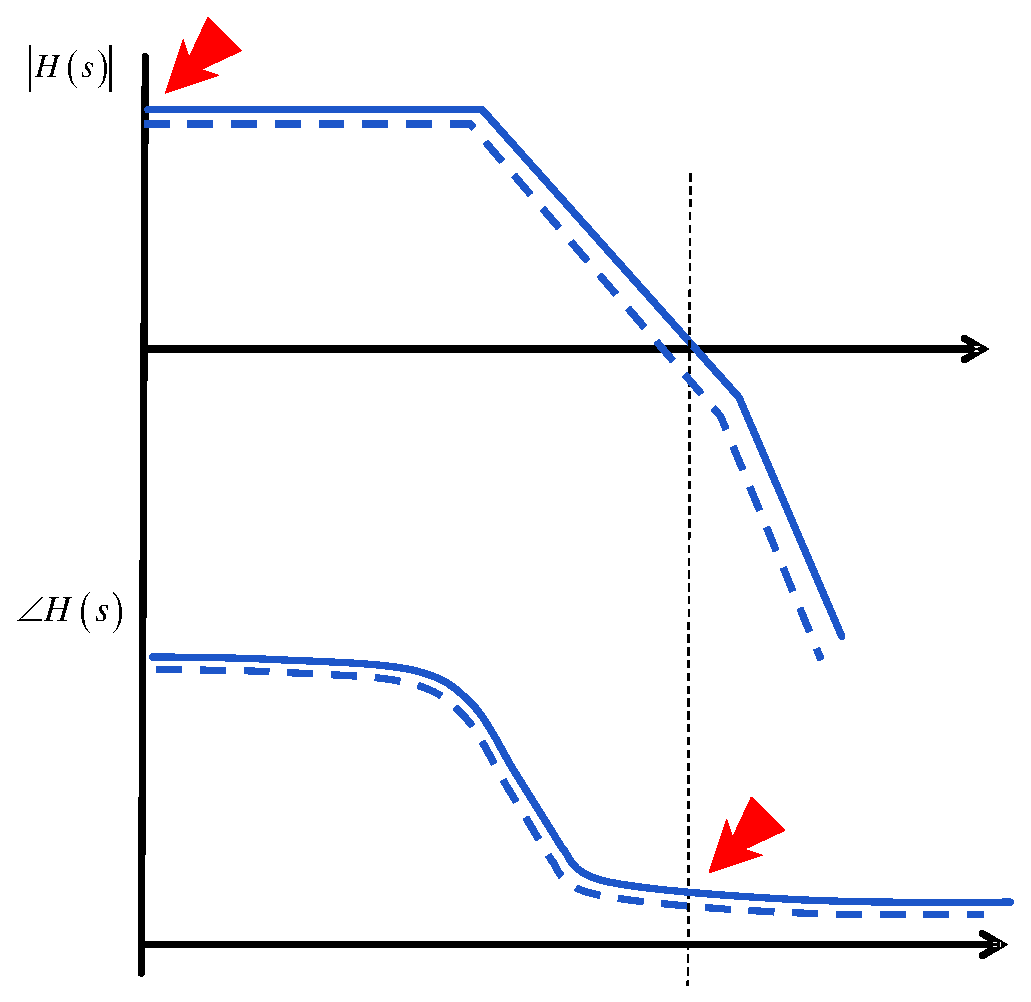
\includegraphics[width=0.7\textwidth]{chap2/significance.eps}
	\bicaption[fig:significance]{元件变化对运放增益和相位裕度的影响}{元件变化对运放增益和相位裕度的影响}{Fig}{The impact of element value on gain and phase margin}
\end{figure}

可以想象,如图\ref{fig:significance},当运放电路元件发生变化的过程中,其相应的差分增益与单位增益频率处的相位会发生变化。
同样,如果一个元件对运放的差分增益贡献较大,那么在把这个元件从电路中以置为无穷大或者零的方式,将其从电路中删去后,电路的频率响应会发生剧烈变动。
也就是说,一个运放的重要性基本等同于元件变化时的电路性能变化的程度。
这一点,正是作为我们选取重要性指标的关键所在。

\begin{figure}[!htp]
	\centering
	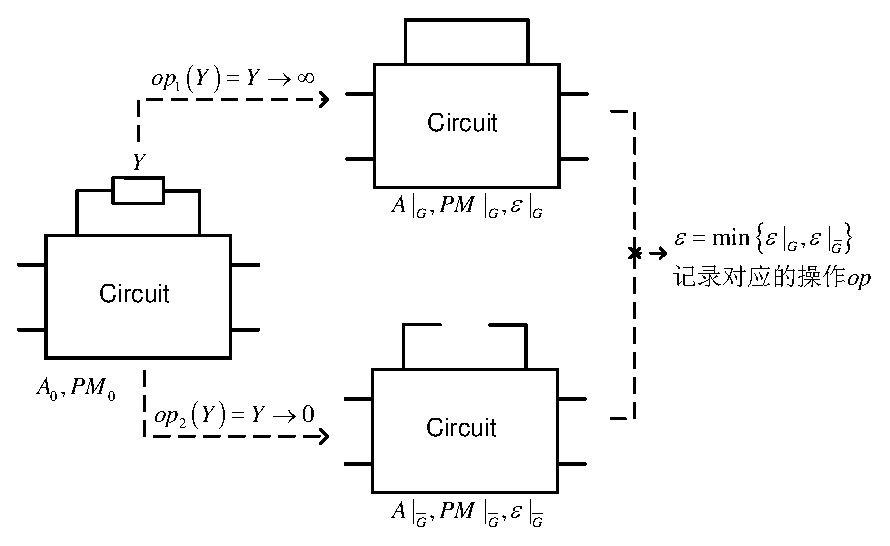
\includegraphics[width=0.8\textwidth]{chap2/SignProcess.eps}
	\bicaption[fig:SignProcess]{元件重要性计算流程}{元件重要性计算流程}{Fig}{Element significance calculation process}
\end{figure}

总结来说,元件重要性计算的整体流程如图\ref{fig:SignProcess}所示。
在算法运行初期,我们得到了运放在一般情况下的差分增益$A_0$以及其在单位频率$UGF$处的相位$PM_0$。
接下来,假设我们需要对电路中的元件$S$求取重要性,那么我们首先将$S$的值置为无穷大,取得此时的运放差分增益$A|_G$以及其在单位频率$UGF$处的相位$PM|_G$,并记录相应的操作为$op1$。
然后,将$S$的值置为零,取得此时的运放差分增益$A|_{\overline G}$以及其在单位频率$UGF$处的相位$PM|_{\overline G}$,并记录相应的操作为$op2$。
在获得了相应的变化之后,我们可以分别计算得到电路在两种情况下分别的电路AC性能的变动指标。
这里我们采用了平方和开根的方式对增益和相位两个指标进行融合。
同时,为了保证两种不同的物理量之间相互能够比较,采用了相对误差的计算方式,如下两式所示:

\begin{equation}
\varepsilon {|_G} = \sqrt {{{\left( {\frac{{A{|_G} - {A_0}}}
				{{{A_0}}}} \right)}^2} + {{\left( {\frac{{PM{|_G} - P{M_0}}}
				{{P{M_0}}}} \right)}^2}}
\end{equation}

\begin{equation}
\varepsilon {|_{\overline G }} = \sqrt {{{\left( {\frac{{A{|_{\overline G }} - {A_0}}}
				{{{A_0}}}} \right)}^2} + {{\left( {\frac{{PM{|_{\overline G }} - P{M_0}}}
				{{P{M_0}}}} \right)}^2}}
\end{equation}

在获得将电路元件置为无穷大和零情况下相应的电路性能的变化$\varepsilon {|_G}$和$\varepsilon {|_{\overline G }}$之后,我们选取其中较小的一个作为之后用于排序的重要性指标$\varepsilon$,同时记得记录对应的删去操作$op$,即如下式:

\begin{equation}
\varepsilon  = \min \left\{ {{\varepsilon {|_G}},{\varepsilon {|_{\overline G }}}} \right\}
\end{equation}

之所以选择较小的$\varepsilon$作为该元件的重要性,主要是因为我们希望在删去电路元件的过程中,应该尽可能小地改变电路的性能指标。
即所选择的$\varepsilon$所对应的删去方式,更适合作为该元件的删去方式,因为删去该元件之后,对电路产生的影响较小。
如有一个电阻,如果其值非常小,可以近似视为短路时,那么明显$\varepsilon {|_G}$会小于$\varepsilon {|_{\overline G }}$,这时应将该电路短路,即选择$\varepsilon {|_G}$作为其重要性,并进行接下来的操作。

可以看到重要性计算过程中需要求取在元件值为零和无穷大时分别的AC增益和$UGF$处的相位,故需要对两种符号情况的两个频率点分别计算电路的传输函数。
这总共需要对GPDD进行4次遍历过程,才可以完成,如忽略常数系数,则重要性计算的时间复杂度约为$\left|GPDD\right|$。

\subsection{简化特殊情况分析}
\label{subsec:simp:alg:special}

在简化过程中,存在两种可能的简化特殊情况,需要区别处理。
出现这些情况的主要原因是对应的电路中拓扑结构不合理造成的。
为了使算法能尽可能稳定运行,在不影响电路性能的情况,尽可能多地删去较多的元件。
应对这些情况做出合适处理,以使算法尽可能稳定。

\subsubsection{元件重要性计算过程中处理}
\label{subsubsec:simp:alg:special:sign}

首先在重要性计算过程中,我们是将电路元件的值置为零或无穷大的情况下,然后计算相应的重要性。
但是有可能出现这样的情况,比如某个电路元件承担了将信号从上一级传递到下一级的职责。
那么我们在计算其重要性过程中,如将其值置为无穷大,那么其输出也为无穷大(在程序中显示其值为INF);
如将其值置为零,那么其输出与输入无关(在程序中显示其值为NAN)。
这两种情况都是我们不期望看到的。所以应规定相应的规则,处理类似情况。我们规定如下规则,处理类似情况:

\begin{enumerate}[label=\emph{\alph*})]
	\item 如没有删去方式会导致对应的重要性$\varepsilon$为INF或者NAN,那么按照\ref{subsec:simp:alg:significance}中的重要性计算方式计算。
	\item 如有仅一种删去方式导致对应的重要性$\varepsilon$为INF或者NAN,那么无论另一种删去方式的重要性$\varepsilon$大小,选择另一种删去方式,并记录重要性。
	\item 如果两种删去方式都会导致对应的重要性$\varepsilon$为INF或者NAN,那么对该元件的操作方式记录为保留,即在后续处理中忽略该元件。
\end{enumerate}

通过这种方式,将有效地避免上述出现的情况。保证算法运行的稳定,尽可能多地删去电路元件,以得到合理的低阶电路模型。

\subsubsection{最终电路图中删去元件过程处理}
\label{subsubsec:simp:alg:special:reduce}

另一种特殊情况发生在最终对电路进行电路图层面的约减过程中。因为在电路图的约减过程中,我们仍然需要监控电路的传输函数变化,来确定最终的小信号简化低阶模型的形式。
有些电路需要多个电路元件删去后,才会出现电路传输函数的计算过程中的异常值(NAN或INF)。
这种情况在GPDD计算中,一种常见的情况是电路出现了孤立节点。
然而由于GPDD的构造过程,是枚举电路生成树对,如果由于简化电路,孤立的节点不会出现生成树中,那么就无法计算对应的GPDD的值。
这种情况往往需要对元件的删去方式进行翻转,因为往往这种情况并不影响最终的传输函数结果。下面用一个例子对这种情况进行说明。

\begin{exmp}
电路中多余元件对GPDD求值的影响
	
\begin{figure}[!htp]
	\centering
	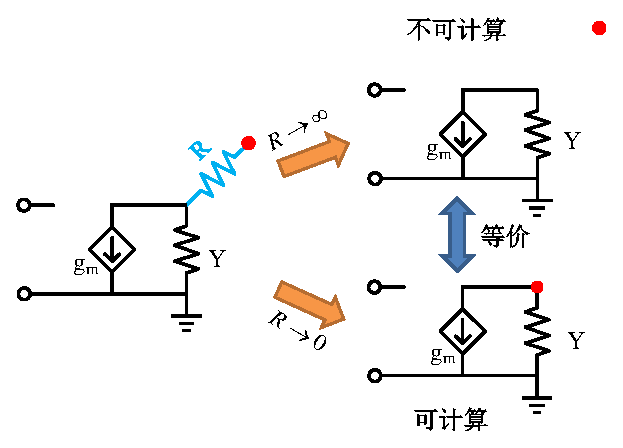
\includegraphics[width=0.6\textwidth]{chap2/CancelCase.eps}
	\bicaption[fig:CancelCase]{电路图约减过程中特殊情况说明}{电路图约减过程中特殊情况说明}{Fig}{Special case in simplified circuit graph reduction}
\end{figure}

可以看到图\ref{fig:CancelCase}中展示了一个多余的电路元件电阻$R$,现在考虑将电阻R删去。
可以看到不论如何删去R都不会影响到电路的传输函数的相应,可是在GPDD中,只有下一种情况是可以继续计算的,因为红色的节点仍然能包含最终的生成树中;
而另一种情况则不包含。这种情况下,GPDD求值存在困难。故如当我们发现类似图\ref{fig:CancelCase}中的情况发生时,及时地改变电路元件的删去方式,那么可以得到可计算的GPDD结构。

\end{exmp}

可以看到只要翻转删去方式,往往可以避免此类的情况的出现;如翻转了仍无效果,可如上一小节\ref{subsubsec:simp:alg:special:sign}中所介绍的一样,保留该元件。
究其深层次的原因,主要是因为GPDD并不完全没有对消项造成的,仍存在类似公因子对消项,这一点会在附录\ref{app:cancel}中给出详细的说明。

\section{降阶模型生成算法测试结果与分析}
\label{sec:simp:res}

\subsection{预处理简化降阶电路模型区别}
\label{subsec:simp:res:pre}

\subsection{多种电路结构简化结果分析}
\label{subsec:simp:res:cir}

\subsubsection{折叠共源共栅运算放大器拓扑简化结果}
\label{subsubsec:simp:res:cir:fd}

\subsubsection{多种补偿结构的两级运算放大器拓扑简化结果}
\label{subsubsec:simp:res:cir:ts}

\subsection{尺寸调整下的算法稳定性分析}
\label{subsec:simp:res:size}

\subsection{简化符号化模型阶数比较}
\label{subsec:simp:res:order}

\section{本章小结}
\label{sec:simp:con}

本章对本文的关键技术符号降阶模型的自动生成进行了详细介绍,并分析了加入各个流程原因以及需要考虑的特殊情况。
通过广泛大量的测试,可以看到本文提出的符号化降阶算法有效地降低了电路模型的阶数,并且得到十分合理、易于电路工程师进行理解的简化电路小信号模型。
这里采用的关键技术为符号化拓扑的简化的方法。这一方法相对于传统的一些符号化简化方法,总结下来,有以下几方面优势:

\begin{enumerate}[label=\emph{\alph*})]
	\item 可以直接给出简化后的电路拓扑结构,易于模拟电路工程师进行分析。
	\item 在过程中,同时得到电路的符号化公式,可直接提供给用户做进一步分析。
	\item 得到的简化结果直接对应于原始电路中的电路元件,有助于做尺寸调整,避免了传统方法中简化结果无法对应会电路的问题。
	\item 区别于传统矩阵降阶方法,是一种启发式的符号化模型降阶方法。
\end{enumerate}